% 1108.tex
% 研究型文章学习笔记模板
% 建议使用 XeLaTeX 编译(支持中文)
\documentclass[11pt,a4paper]{article}
\usepackage[margin=2.5cm]{geometry}
\usepackage{fontspec}
\usepackage{xeCJK}
\usepackage{amsmath,amssymb}
\usepackage{bm}
\usepackage{graphicx}
\usepackage{float}
\usepackage{caption}
\usepackage{booktabs}
\usepackage{enumitem}
\usepackage[colorlinks=true,linkcolor=blue,citecolor=blue,urlcolor=blue]{hyperref}
\usepackage{fancyhdr}
\usepackage{tcolorbox}
\usepackage{datetime}

% 字体(可按需修改)
\setmainfont{TeX Gyre Termes}
\setCJKmainfont{SimSun} % Windows 常见中文字体,视系统调整

% 页眉页脚
\pagestyle{fancy}
\fancyhf{}
% \lhead{\small 研究笔记}
\rhead{\small \PaperMeta}
\cfoot{\small \thepage}

% 元数据命令(在文档开始处填写)
\newcommand{\PaperMeta}{}
\newcommand{\PaperTitle}{}
\newcommand{\PaperAuthors}{}
\newcommand{\PaperVenue}{}
\newcommand{\PaperYear}{}
\newcommand{\PaperLink}{}

% 强调框
\newtcolorbox{highlight}{colback=yellow!10,colframe=yellow!60!black,boxrule=0.5pt}

\begin{document}

% ————— 填写元数据 —————
\renewcommand{\PaperTitle}{Observation and Modulation of the Quantum Mpemba Effect on a Superconducting Quantum Processor}
\renewcommand{\PaperAuthors}{Yueshan Xu, Cai-Ping Fang, Bing-Jie Chen, Ming-Chuan Wang}
\renewcommand{\PaperVenue}{ArXiv}
\renewcommand{\PaperYear}{2025}
\renewcommand{\PaperLink}{http://arxiv.org/abs/2508.07707}
\renewcommand{\PaperMeta}{\PaperTitle\ --- \PaperYear}

% ————— 路径设置 —————
\newcommand{\paperpath}{D:/B_Dr/arXiv-2508.07707v1/}
\graphicspath{{\paperpath}}

\begin{center}
    {\LARGE \textcolor{blue}{\PaperTitle}}\\[6pt]
    {\small \PaperAuthors \quad | \quad \PaperVenue \quad | \quad \PaperYear}\\
    {\small \url{\PaperLink}}
\end{center}

\tableofcontents
\vspace{6pt}
\hrule
\vspace{10pt}

% ————— 快速摘要 —————
\section*{快速摘要(TL;DR)}

Can we leverage the flexibility of our systemsuch as varied on-site potentials and diverse initial states-to recover QME in the intermediate-coupling regime?



\section{背景介绍}
\begin{enumerate}[leftmargin=*]
    \item In non-equilibrium quantum many-body systems, the quantum Mpemba effect (QME) emerges as a counterintuitive phenomenon: systems exhibiting greater initial symmetry breaking restore symmetry faster than those with less.
    \item \textcolor{blue}{Three major research fields}
        \begin{itemize}
        \item The Mpemba effect, originally observed as faster freezing of hotter water than colder water under identical conditions, represents a counterintuitive non-equilibrium phenomenon with debated mechanisms.
        \item In open quantum systems interacting with an external environment through Markovian and non-Markovian processes. It is dominated by classical fluctuations, resembling the classical Mpemba effect
        \item In isolated quantum systems governed by intrinsic quantum dynamics. It is driven by intrinsic quantum fluctuations. \textcolor{blue}{In isolated quantum systems, the quantum Mpemba effect (QME) manifests as a remarkable phenomenon: subsystems with greater initial symmetry breaking restore symmetry faster under a symmetry-preserving Hamiltonian.} The type of system under the study:
        \begin{itemize}
            \item Quasiparticle framework for integrable systems that include 1D or 2D models.
            \item In chaotic systems using random and dualunitary circuits.
            \item Non-ergodic contexts, such as many-body localized (MBL) systems
            \end{itemize}
        \end{itemize}
    \item 伪代码/核心算法要点
\end{enumerate}


\section{实验方案}
\begin{enumerate}
    \item Here, we report the observation and control of QME using a superconducting processor featuring a unique fully connected, tunable-coupling architecture that enables precise modulation from short- to long-range interactions.
    \item 调控参量
        \begin{enumerate}
            \item interaction range
            \item potential engineering 
            \item initial state selection
        \end{enumerate}
\end{enumerate}

\subsection{哈密顿量}


实验系统由 16 个超导量子比特组成,采用全连接环状拓扑结构,具备可调耦合能力。系统的有效哈密顿量可写为:

\begin{equation}
H = \sum_{i < j} g_{ij} (\sigma^{+}_{i} \sigma^{-}_{j} + \sigma^{-}_{i} \sigma^{+}_{j}) + \sum_{i} h_i \sigma^{+}_{i} \sigma^{-}_{i}
\end{equation}

其中:
\begin{itemize}
    \item $g_{ij}/2\pi$ 表示量子比特 $Q_i$ 与 $Q_j$ 之间的耦合强度;
    \item $\sigma^{+}_{i}$ 和 $\sigma^{-}_{i}$ 分别为第 $i$ 个量子比特的升降算符;
    \item $h_i/2\pi$ 表示通过频率调制实现的在位势能,参考频率为 $\omega_{\text{ref}}/2\pi \approx 4.24\ \text{GHz}$。
\end{itemize}

为了区分不同耦合范围,我们将耦合强度分为两部分:
\begin{equation}
\begin{aligned}
H &= \sum_{i, j=i+1} g_N (\sigma^{+}_{i} \sigma^{-}_{j} + \sigma^{-}_{i} \sigma^{+}_{j}) \\
&\quad + \sum_{i < j, j \neq i+1} g_L (\sigma^{+}_{i} \sigma^{-}_{j} + \sigma^{-}_{i} \sigma^{+}_{j}) + \sum_{i} h_i \sigma^{+}_{i} \sigma^{-}_{i}
\end{aligned}
\end{equation}

其中:
\begin{itemize}
    \item $g_N/2\pi$ 表示最近邻(短程)耦合强度;
    \item $g_L/2\pi$ 表示长程耦合强度。
\end{itemize}

定义耦合比 $r = |g_N / g_L|$,用于量化不同相互作用区间:
\begin{itemize}
    \item $r \gg 1$:强短程耦合区间;
    \item $r \approx 1$:中间耦合区间;
    \item $r \ll 1$:弱短程耦合区间。
\end{itemize}

通过调节中心总线谐振器频率 $\Delta_{RQ}$ 和耦合器频率 $\Delta_{CQ}$ 相对于参考频率的失谐,可实现 $r$ 的连续调控。



% ————— 图1:量子处理器显微照片和耦合强度调制 —————
\section{实验装置与耦合调控}

\begin{figure}[H]
    \centering
    \includegraphics[width=0.95\textwidth]{Figure1/Figure1.pdf}
    \caption{
        \textcolor{blue}{量子处理器的显微照片和耦合强度调制。}
        (a) 超导量子处理器的光学显微照片,采用环状拓扑结构,包含16个量子比特,通过16个可调耦合器($C$)和中心总线谐振器($R$)互连。插图为谐振器中心约瑟夫森结的光学显微照片。
        (b) 实验协议的脉冲序列,通过$R$和$C$实现耦合强度的灵活调制。协议包括:在倾斜乘积态中初始化系统,使用Z脉冲将量子比特调至工作点(施加各种在位势),通过多量子比特量子态层析构建子系统$A=\{Q_1,Q_2,Q_3\}$的密度矩阵。
        (c,d) 有效耦合强度$g/2\pi$示意图,分别对应$r\approx 10$和$r\approx 1$,其中$r$为最近邻与长程耦合强度之比。线宽和颜色表示$g/2\pi$的大小。
    }
    \label{fig:device_and_coupling}
\end{figure}

\textcolor{blue}{关键参数说明:}
\begin{itemize}
    \item \textcolor{blue}{处理器架构:} 16量子比特全连接环状拓扑,每个量子比特电容耦合至最近邻耦合器,同时所有量子比特电容耦合至中心频率可调总线谐振器(4.5–6.5 GHz)
    \item \textcolor{blue}{实验选择:} 实验中选用14个相邻量子比特组成紧密连接链状阵列
    \item \textcolor{blue}{耦合调控:} 通过调节中心总线谐振器频率$\Delta_{RQ}$和耦合器频率$\Delta_{CQ}$实现不同耦合区间:
    \begin{itemize}
        \item 强短程耦合区间($r\approx 10$):$\Delta_{CQ}\approx 1.0$ GHz,$\Delta_{RQ}\approx 2.2$ GHz
        \item 中间耦合区间($r\approx 1$):$\Delta_{CQ}\approx 2.0$ GHz,$\Delta_{RQ}\approx 0.4$ GHz
    \end{itemize}
\end{itemize}

\textcolor{blue}{三种在位势:}
\begin{itemize}
    \item 无在位势:$h_i = 0$,所有量子比特调谐到相同的频率,所有量子比特"共振",能量均匀分布。\textcolor{red}{共振 ($h_i=0$):完美能量匹配 $\rightarrow$ 高效的能量传递 $\rightarrow$ 快速热化}
    \item 线性在位势:$h_i = \omega_{\text{ref}}/2\pi$,施加位置依赖的线性梯度场。\textcolor{red}{线性 ($h_i$ 线性变化):系统性失配 $\rightarrow$ 抑制热化,诱导局域化}
    \item 无序在位势:$h_i = \omega_{\text{ref}}/2\pi \cos(2\pi i t)$,每个量子比特施加随机的在位势。\textcolor{red}{非线性 ($h_i$ 随机变化):随机失配 $\rightarrow$ 破坏相干性,减缓弛豫}
\end{itemize}


\section{结论}
\begin{enumerate}
    \item In strong \textcolor{blue}{short-range} coupling regimes, EA crossovers during quenches from \textcolor{blue}{tilted Néel states} confirm the presence of QME.
    \item In \textcolor{blue}{intermediate coupling regimes}, \textcolor{red}{synchronized EA and entanglement entropy} dynamics reveal the \textcolor{blue}{suppression} of QME.
    \item QME reemerges with the introduction of \textcolor{red}{on-site linear potentials or quenches from tilted ferromagnetic states}, the latter proving robust against on-site disorder.
\end{enumerate}

% \section{各EA图的实验条件梳理}

\subsection{实验参数总结}

\begin{table}[H]
\centering
\caption{各EA图的实验调制参数总结}
\begin{tabular}{|c|c|c|c|c|}
\hline
\textbf{图号} & \textbf{初始态类型} & \textbf{相互作用范围} & \textbf{在位势类型} & \textbf{主要物理现象} \\
\hline
\textbf{图2c} & 倾斜Néel态 & 强短程耦合 ($r \approx 10$) & 共振 ($h_i = 0$) & QME出现(EA交叉) \\
\hline
\textbf{图3a} & 倾斜Néel态 & 中间耦合 ($r \approx 1$) & 共振 ($h_i = 0$) & QME抑制(无EA交叉) \\
\hline
\textbf{图3b} & 倾斜Néel态 & 中间耦合 ($r \approx 1$) & 线性势 ($W = 6$ MHz) & QME重现(EA交叉) \\
\hline
\textbf{图4a} & 倾斜铁磁态 & 中间耦合 ($r \approx 1$) & 共振 ($h_i = 0$) & QME重现(EA交叉+振荡) \\
\hline
\textbf{图4c} & 倾斜铁磁态 & 中间耦合 ($r \approx 1$) & 无序 ($h_i \in [-14\bar{g},14\bar{g}]$) & QME鲁棒性(EA交叉保持) \\
\hline
\end{tabular}
\end{table}

\subsection{详细参数分析}

\subsubsection{图2c:强短程耦合区间的QME}
\begin{itemize}
    \item \textbf{初始态}:倾斜Néel态 $|\theta\rangle_N$,$\theta = \pi/4$ 和 $\pi/2$
    \item \textbf{耦合参数}:
    \begin{itemize}
        \item 最近邻耦合:$g_N/2\pi = -5$ MHz
        \item 长程耦合:$g_L/2\pi \approx 0.5$ MHz
        \item 耦合比:$r \approx 10$
    \end{itemize}
    \item \textbf{在位势}:共振条件(所有量子比特调至$\omega_{\text{ref}}$)
    \item \textbf{物理机制}:准粒子介导的弛豫,大倾斜角激发快速传播模式
\end{itemize}

\subsubsection{图3a:中间耦合区间的QME抑制}
\begin{itemize}
    \item \textbf{初始态}:倾斜Néel态 $|\theta\rangle_N$,$\theta = \pi/4$ 和 $\pi/2$
    \item \textbf{耦合参数}:
    \begin{itemize}
        \item 最近邻耦合:$g_N/2\pi = -2$ MHz
        \item 长程耦合:$g_L/2\pi \approx -2$ MHz
        \item 耦合比:$r \approx 1$
    \end{itemize}
    \item \textbf{在位势}:共振条件
    \item \textbf{物理机制}:热化主导动力学,小倾斜角热化更快
\end{itemize}

\subsubsection{图3b:线性势诱导的QME重现}
\begin{itemize}
    \item \textbf{初始态}:倾斜Néel态 $|\theta\rangle_N$,$\theta = \pi/4$ 和 $\pi/2$
    \item \textbf{耦合参数}:中间耦合 ($r \approx 1$)
    \item \textbf{在位势}:线性势 $h_j/2\pi = W(7.5 - j)$,$W = 6$ MHz
    \item \textbf{物理机制}:线性势抑制热化,诱导类似Stark局域化行为
\end{itemize}

\subsubsection{图4a:铁磁态淬火的QME重现}
\begin{itemize}
    \item \textbf{初始态}:倾斜铁磁态 $|\theta\rangle_F$,$\theta = \pi/4$ 和 $\pi/2$
    \item \textbf{耦合参数}:中间耦合 ($r \approx 1$)
    \item \textbf{在位势}:共振条件
    \item \textbf{物理机制}:映射到可积LMG模型,集体自旋动力学
    \item \textbf{特殊现象}:EA振荡,周期$T_{\text{EA}} = \pi/\bar{g}$
\end{itemize}

\subsubsection{图4c:无序势下的QME鲁棒性}
\begin{itemize}
    \item \textbf{初始态}:倾斜铁磁态 $|\theta\rangle_F$,$\theta = \pi/4$ 和 $\pi/2$
    \item \textbf{耦合参数}:中间耦合 ($r \approx 1$)
    \item \textbf{在位势}:无序势,$h_i/2\pi$从$[-14\bar{g},14\bar{g}]$均匀采样
    \item \textbf{物理机制}:无序破坏集体行为但保持QME,显示鲁棒性
\end{itemize}

\subsection{实验设计的系统性与对比性}

\subsubsection{初始态类型的对比}
\begin{table}[H]
\centering
\caption{不同初始态的对比研究}
\begin{tabular}{|c|c|c|}
\hline
\textbf{耦合区间} & \textbf{Néel态结果} & \textbf{铁磁态结果} \\
\hline
强短程耦合 & 图2c:QME出现 & 未展示 \\
\hline
中间耦合+共振 & 图3a:QME抑制 & 图4a:QME重现 \\
\hline
中间耦合+势场 & 图3b:QME重现(线性势) & 图4c:QME鲁棒(无序) \\
\hline
\end{tabular}
\end{table}

\subsubsection{耦合区间的系统研究}
\begin{itemize}
    \item \textbf{强短程耦合 ($r \approx 10$)}:近可积动力学,准粒子机制主导
    \item \textbf{中间耦合 ($r \approx 1$)}:热化主导,但可通过势场调控
    \item \textbf{实验覆盖}:从近可积到热化的完整相图
\end{itemize}

\subsubsection{在位势的多维调控}
\begin{table}[H]
\centering
\caption{不同在位势的调控效果}
\begin{tabular}{|c|c|c|}
\hline
\textbf{在位势类型} & \textbf{对热化的影响} & \textbf{对QME的影响} \\
\hline
共振 ($h_i = 0$) & 促进热化 & 在中间耦合抑制QME \\
\hline
线性势 ($h_j = W(7.5-j)$) & 抑制热化,诱导局域化 & 重现QME \\
\hline
无序势 ($h_i$随机) & 抑制热化,破坏集体行为 & QME保持鲁棒 \\
\hline
\end{tabular}
\end{table}

\subsection{物理洞察与意义}

\subsubsection{QME出现的条件}
\begin{itemize}
    \item \textbf{必要条件}:对称的动力学 ($[H,Q_A]=0$) + 不对称的初始态
    \item \textbf{充分条件}:
    \begin{itemize}
        \item 可积性主导(强短程耦合)
        \item 或热化被抑制(通过势场工程)
        \item 且不同倾斜角的对称性恢复速率关系反常
    \end{itemize}
\end{itemize}

\subsubsection{实验设计的深层逻辑}
\begin{itemize}
    \item \textbf{系统性}:通过三个独立变量(初始态、耦合、势场)的系统扫描
    \item \textbf{对比性}:每个变量都在不同条件下对比研究
    \item \textbf{完备性}:覆盖了从可积到热化再到局域化的完整非平衡动力学相图
\end{itemize}

\subsubsection{技术成就展示}
\begin{itemize}
    \item \textbf{哈密顿量工程}:精确调控耦合强度和范围
    \item \textbf{态制备}:高保真度制备不同初始态
    \item \textbf{动力学测量}:通过QST和EA量化对称性恢复
    \item \textbf{参数空间探索}:多维参数空间的系统扫描能力
\end{itemize}

\subsection{总结}

这篇文献通过精心设计的实验,系统性地探索了量子Mpemba效应在不同参数空间中的行为,展示了超导量子处理器在量子多体非平衡动力学研究中的强大能力。实验设计具有高度的系统性和对比性,为理解QME的普适性和可控性提供了坚实基础。


\section{关键公式与推导}
Entanglement asymmetry (EA), defined as the relative entropy
\begin{equation}
\Delta S_A(t)=S\left(\rho_{A, Q}(t)\right)-S\left(\rho_A(t)\right)
\end{equation}
where $\rho_A$ is the reduced density matrix of subsystem $A$, $\rho_{A, Q}=\sum_q \Pi_q \rho_A \Pi_q$ denotes its projection onto the \textcolor{red}{conserved charge $Q_A$ eigenspaces}, and $S\left(\rho_A\right)$ is the von Neumann entropy of $\rho_A$. 

$\Delta S_A(t)$ captures the distance of $\rho_A$ from a \textcolor{red}{symmetric state $\rho_A,Q$} including contributions from non-local correlations within subsystem A that violate the symmetry.

This makes it a natural \textcolor{blue}{order parameter} for non-equilibrium dynamics, offering a fresh perspective on thermalization compared to traditional metrics like entanglement entropy.


% ————— 实验设置 —————
% \section{实验与结果}

% ————— 图2:EA测量实验协议及强短程耦合区间的EA动力学 —————
\section{短程相互作用区间的纠缠不对称性测量与QME观测}

\begin{figure}[H]
    \centering
    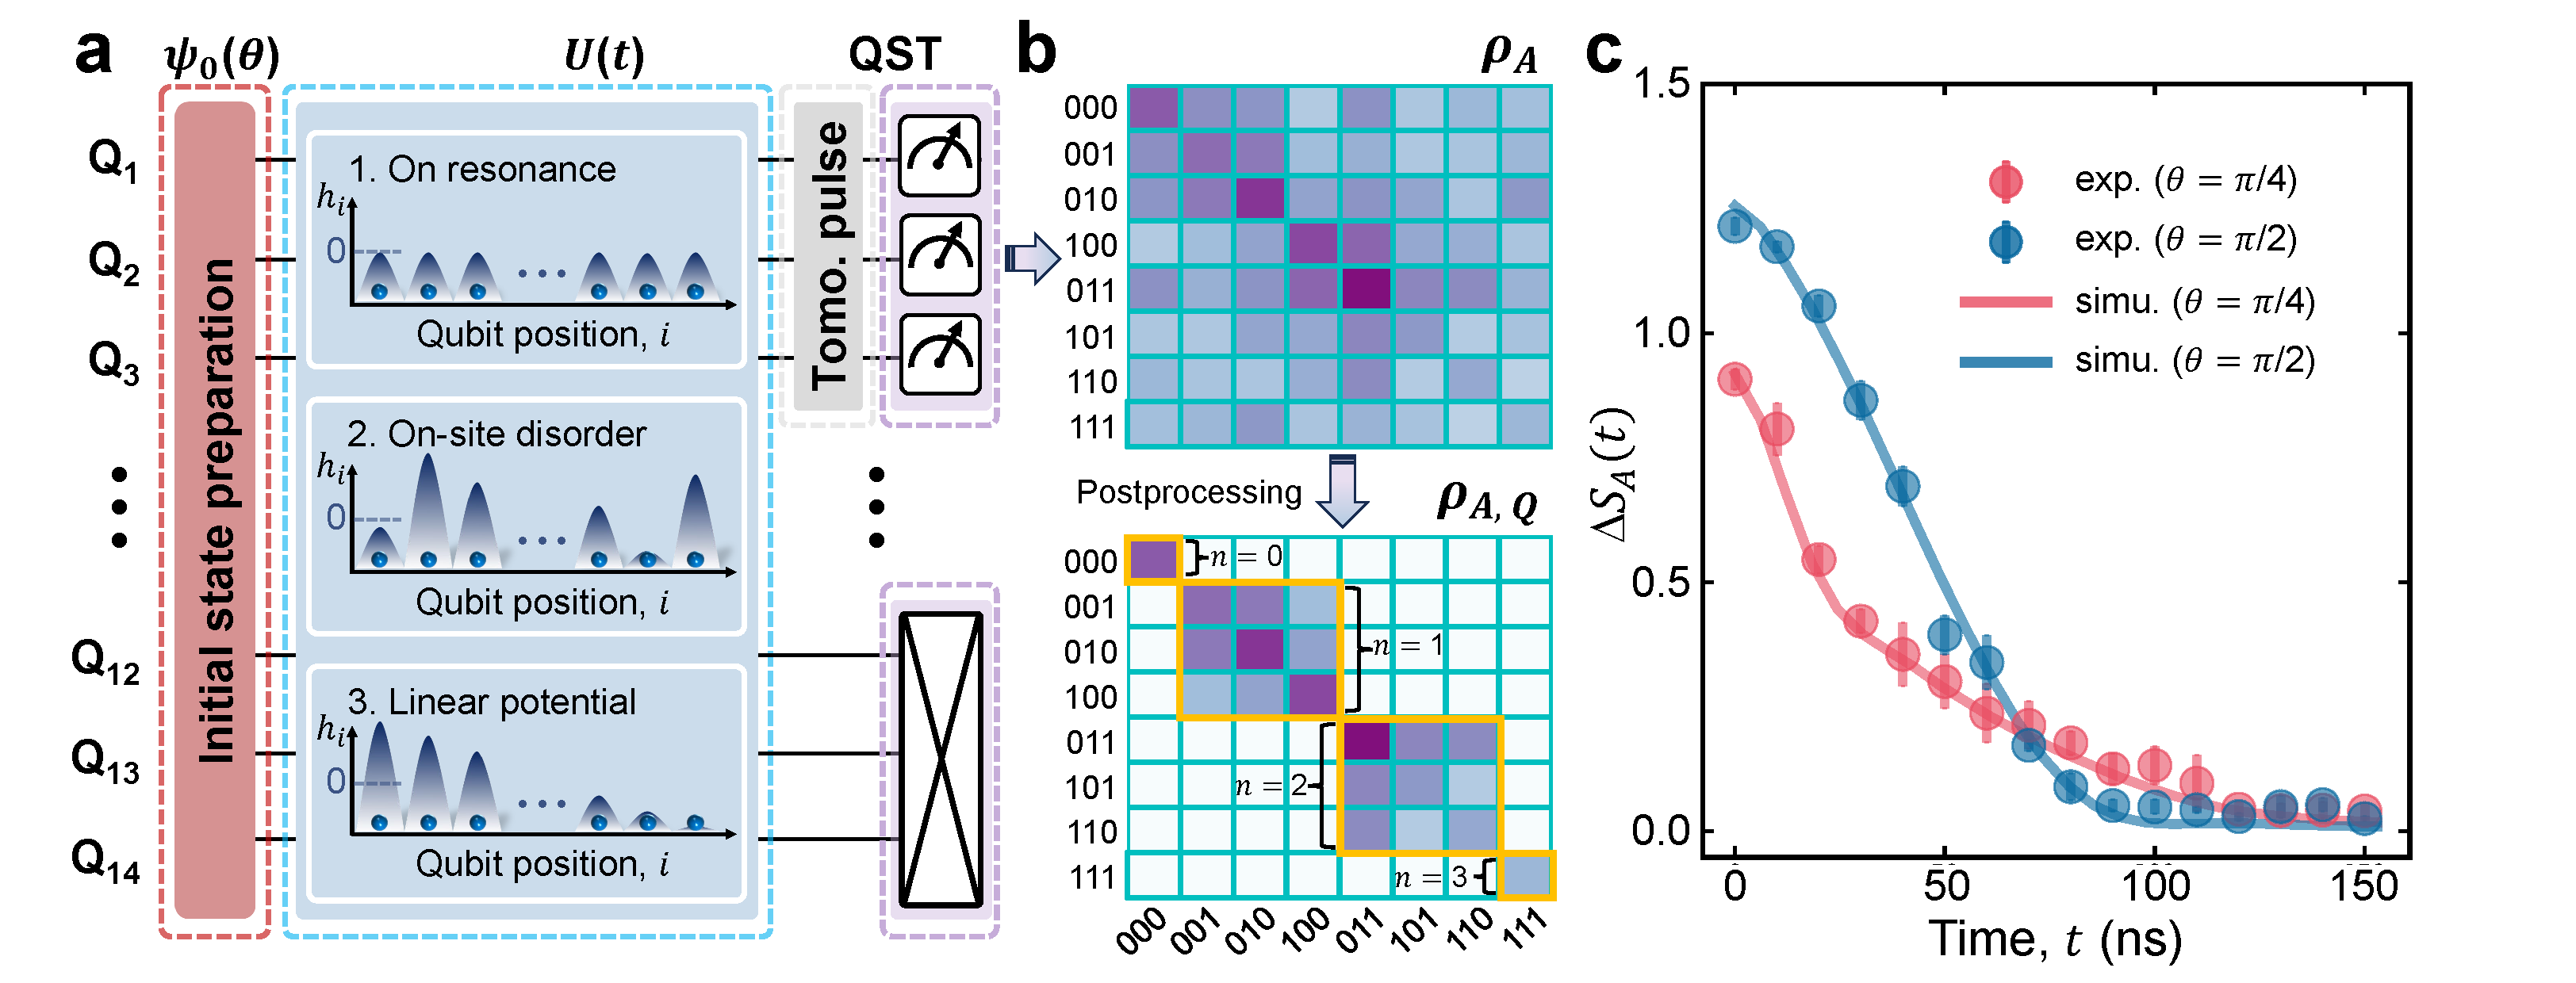
\includegraphics[width=0.95\textwidth]{Figure2/Figure2.pdf}
    \caption{
        \textcolor{blue}{强短程耦合区间($r\approx 10$)EA测量实验协议及其动力学。}
        (a) 实验协议的量子电路图。在初始态$|\Psi(\theta)\rangle$制备后,系统在工程化哈密顿量$H$下演化:$|\Psi(t)\rangle = U(t)|\Psi(\theta)\rangle = e^{-iHt}|\Psi(\theta)\rangle$,其中对量子比特施加了不同类型的在位势(共振、无序或线性梯度场)。
        (b) 通过量子态层析重建子系统$A$的密度矩阵。将密度矩阵投影到电荷算符$Q_A$的本征空间后,应用经典后处理来估计EA。
        (c) 强短程耦合区间($r\approx 10$)下量子比特共振时,倾斜Néel初始态(角度$\theta=\pi/4$和$\pi/2$)的EA动力学。观察到$\theta=\pi/2$时对称性恢复更快,并出现明显的交叉现象,证实了QME的存在。符号为实验数据,实线为包含退相干的理论结果。误差棒表示10次实验重复的标准偏差,每次包含3000次测量。
    }
    \label{fig:EA_measurement_strong_coupling}
\end{figure}

\textcolor{blue}{关于$\rho_A$和$\rho_{A, Q}$的深入理解:}
\begin{enumerate}
    \item \textcolor{blue}{约化密度矩阵 $\rho_A$}
    \begin{itemize}
        \item \textcolor{blue}{定义:} $\rho_A$ 是子系统 $A = \{Q_1, Q_2, Q_3\}$ 的约化密度矩阵,通过对总系统(14个量子比特)的密度矩阵 $\rho_{\text{total}}$ 对补集 $\bar{A} = \{Q_4, Q_5, \dots, Q_{14}\}$ 取部分迹得到:
        \begin{equation}
        \rho_A = \operatorname{Tr}_{\bar{A}} (\rho_{\text{total}})
        \end{equation}
        
        \item \textcolor{blue}{数学表示:} 在计算基下,$\rho_A$ 是一个 $8 \times 8$ 的厄米矩阵,满足:
        \begin{itemize}
            \item 半正定性:$\rho_A \succeq 0$
            \item 迹为1:$\operatorname{Tr}(\rho_A) = 1$
            \item 矩阵元 $\rho_{ij} = \langle i | \rho_A | j \rangle$,其中 $i,j \in \{000,001,\dots,111\}$
        \end{itemize}
        
        \item \textcolor{blue}{物理意义:} $\rho_A$ 完整描述了子系统 $A$ 的量子态,包含:
        \begin{itemize}
            \item 对角元:各个计算基态的概率分布
            \item 非对角元:不同基态间的量子相干性
        \end{itemize}
    \end{itemize}
    
    \item \textcolor{blue}{投影密度矩阵 $\rho_{A,Q}$}
    \begin{itemize}
        \item \textcolor{blue}{定义:} $\rho_{A,Q}$ 是 $\rho_A$ 在守恒荷 $Q_A = \sum_{i\in A} \sigma_z^i$ 的本征空间上的投影:
        \begin{equation}
        \rho_{A,Q} = \sum_{q} \Pi_q \rho_A \Pi_q
        \end{equation}
        其中 $\Pi_q$ 是投影到本征值 $q$ 对应子空间的投影算符。
        
        \item \textcolor{blue}{本征值分组:} 对于3量子比特系统,$Q_A$ 的本征值为激发数($|1\rangle$ 的个数):
        \begin{align*}
        q = 0 &: \{|000\rangle\} \quad \text{(1维)} \\
        q = 1 &: \{|001\rangle, |010\rangle, |100\rangle\} \quad \text{(3维)} \\
        q = 2 &: \{|011\rangle, |101\rangle, |110\rangle\} \quad \text{(3维)} \\
        q = 3 &: \{|111\rangle\} \quad \text{(1维)}
        \end{align*}
        
        \item \textcolor{blue}{矩阵结构:} 在计算基排序下,$\rho_{A,Q}$ 具有块对角形式:
        \begin{equation}
        \rho_{A,Q} = \begin{pmatrix}
        \text{块}_0 & 0 & 0 & 0 \\
        0 & \text{块}_1 & 0 & 0 \\
        0 & 0 & \text{块}_2 & 0 \\
        0 & 0 & 0 & \text{块}_3
        \end{pmatrix}
        \end{equation}
        其中每个块对应一个电荷子空间。
        
        \item \textcolor{blue}{物理意义:} \textcolor{red}{投影操作消除了不同电荷子空间之间的量子相干性,只保留每个电荷子空间内部的量子特性。}这使得 $\rho_{A,Q}$ 成为一个 $U(1)$ 对称的状态。
    \end{itemize}
    
    \item \textcolor{blue}{关键区别与联系}
    \begin{itemize}
        \item $\rho_A$ 可能破坏 $U(1)$ 对称性,包含不同电荷子空间间的相干项
        \item $\rho_{A,Q}$ 严格保持 $U(1)$ 对称性,不同电荷子空间间无相干性
        \item 纠缠不对称性 $\Delta S_A = S(\rho_{A,Q}) - S(\rho_A)$ 量化了对称性破缺的程度:
        \begin{itemize}
            \item $\Delta S_A = 0$:状态具有 $U(1)$ 对称性
            \item $\Delta S_A > 0$:状态破坏 $U(1)$ 对称性
        \end{itemize}
    \end{itemize}
\end{enumerate}
\textcolor{blue}{两个层面的对称性与量子Mpemba效应机制}

\subsection{对称性的两个层面}
\begin{enumerate}
    \item \textcolor{blue}{动力学对称性}:$[H, Q_A] = 0$,保证电荷守恒
    \begin{itemize}
        \item \textcolor{red}{核心关系}:算符与哈密顿量对易 $\rightarrow$ 该算符对应的物理量是守恒量,哈密顿量具有该算符生成的对称性(例如 $U(1)$ 对称性)
        \item \textcolor{blue}{数学表达}:如果 $[H, Q] = 0$,那么 $e^{-iHt} Q e^{iHt} = Q$
        \item \textcolor{blue}{深层含义}:哈密顿量在对称变换下不变,$H = U^\dagger(\phi) H U(\phi)$
    \end{itemize}

    \item \textcolor{blue}{状态对称性}:$[\rho, Q_A] = 0$,状态本身具有对称性
    \begin{itemize}
        \item \textcolor{blue}{物理意义}:状态本身具有对称性
        \item \textcolor{blue}{数学表达}:如果 $[\rho, Q] = 0$,那么 $\rho$ 在对称变换下不变,$\rho = U^\dagger(\phi) \rho U(\phi)$
        \item \textcolor{blue}{量子态特征}:状态是电荷本征态的混合或叠加,但不包含不同电荷间的相干性
    \end{itemize}
\end{enumerate}

\subsection{量子Mpemba效应的核心机制}
\begin{itemize}
    \item \textcolor{blue}{关键现象}:即使动力学是对称的($[H, Q_A] = 0$),初始状态 $\rho_A(0)$ 也可能破坏对称性,然后在演化过程中逐渐恢复对称性
    
    \item \textcolor{blue}{两种演化路径}:
    \begin{itemize}
        \item 对称的动力学 + 不对称的初始状态 $\rightarrow$ 对称性恢复过程
        \item 对称的动力学 + 对称的初始状态 $\rightarrow$ 始终保持对称性
    \end{itemize}
    
    \item \textcolor{blue}{$U(1)$ 对称性定义}:系统在绕 $z$ 轴的任意旋转下不变
\end{itemize}

\subsection{强短程耦合区间的QME机制:准粒子介导的弛豫}
\begin{itemize}
    \item \textcolor{blue}{理论基础}:在近可积的强短程耦合体系中,QME的出现可以由准粒子图像完美解释
    
    \item \textcolor{blue}{准粒子特性}:
    \begin{itemize}
        \item 可积系统存在稳定的准粒子,作为系统的集体激发
        \item 准粒子在整个演化过程中几乎不衰变
        \item 系统演化时在整个系统中产生纠缠的准粒子对
    \end{itemize}
    
    \item \textcolor{blue}{与纠缠不对称性的关系}:
    \begin{itemize}
        \item 只有子系统 $A$ 内部产生的准粒子对才对 $\Delta S_A$ 有贡献
        \item 准粒子离开子系统 $A$ 后不再贡献于内部的对称性破缺
    \end{itemize}
    
    \item \textcolor{blue}{倾斜角 $\theta$ 的关键作用}:
    \begin{itemize}
        \item \textcolor{blue}{大倾斜角 ($\theta = \pi/2$)}:初始态具有更大对称性破缺,优先激发传播速度更快的准粒子模式
        \item \textcolor{blue}{小倾斜角 ($\theta = \pi/4$)}:对称性破缺较小,激发的准粒子中慢速模式比重更高
        \item \textcolor{blue}{结果}:大倾斜角态虽然初始不对称性更强,但通过快速准粒子更快地恢复对称性,产生QME交叉现象
    \end{itemize}
\end{itemize}




\subsection{实验细节与关键发现:}
\begin{itemize}
    \item \textcolor{blue}{初始态制备:} 倾斜Néel态$|\theta\rangle_N = \bigotimes_{j=1}^{14} R_y(\theta)|s_j\rangle$,其中$|s_j\rangle = |0\rangle$($j$为奇数)或$|1\rangle$($j$为偶数)
    \item \textcolor{blue}{对称性破缺程度:} 倾斜角$\theta$控制全局$U(1)$对称性破缺程度:
    \begin{itemize}
        \item $\theta=0$或$\pi$:所有自旋沿$\sigma_z$方向排列(完全对称)
        \item $\theta=\pi/2$:所有自旋沿$\sigma_x$方向排列(最大对称性破缺)
    \end{itemize}
    \item \textcolor{blue}{耦合参数:} 
    \begin{itemize}
        \item 最近邻耦合:$g_N/2\pi = -5$ MHz
        \item 长程耦合:$g_L/2\pi \approx 0.5$ MHz
        \item 耦合比:$r \approx 10$
    \end{itemize}
    \item \textcolor{blue}{QME特征:} 虽然$|\theta=\pi/2\rangle_N$的初始EA高于$|\theta=\pi/4\rangle_N$,但其更快的对称性恢复导致更快的衰减率,产生明显的交叉现象
    \item \textcolor{blue}{物理机制:} 源于准粒子介导的弛豫,较大倾斜角$\theta$优先激发传播更快的模式,从而加速对称性恢复
\end{itemize}

\subsection{纠缠不对称性定义:}
\begin{equation}
\Delta S_A(t) = S(\rho_{A,Q}(t)) - S(\rho_A(t))
\end{equation}
其中:
\begin{itemize}
    \item $\rho_A$:子系统$A$的约化密度矩阵
    \item $\rho_{A,Q} = \sum_q \Pi_q \rho_A \Pi_q$:在守恒荷$Q_A$本征空间上的投影
    \item $S(\rho)$:冯·诺依曼熵
\end{itemize}


\section{QME在中间耦合区间的抑制}
Investigate the sensitivity of QME to \textcolor{red}{thermalization processes.}

\subsection{辨析可积与热化}
\begin{enumerate}
\item 可积$\rightarrow$不可热化
\item 不可积+无局域化$\rightarrow$通常可以热化(满足本征态热化假设ETH)
\item 不可积 + 强无序 $\rightarrow$ 可能多体局域化MBL(不热化)(有无穷多个局域守恒量,满足的是面积律,保持初态记忆)(强无序破坏共振条件,能量不匹配抑制跃迁)
\end{enumerate}


\subsection{实验设置与参数}
\begin{itemize}
    \item \textcolor{blue}{耦合区间}:中间耦合区间($r \approx 1$)
    \item \textcolor{blue}{耦合参数}:
    \begin{itemize}
        \item 最近邻耦合:$g_N/2\pi = -2$ MHz
        \item 长程耦合:$g_L/2\pi \approx -2$ MHz
        \item 耦合比:$r = |g_N/g_L| \approx 1$
    \end{itemize}
    \item \textcolor{blue}{在位势}:共振条件(所有量子比特调至$\omega_{\text{ref}}/2\pi \approx 4.24$ GHz)
    \item \textcolor{blue}{初始态}:与强短程耦合区间相同的倾斜Néel态($\theta = \pi/4$和$\pi/2$)
\end{itemize}

\subsection{关键实验结果}
\begin{figure}[H]
    \centering
    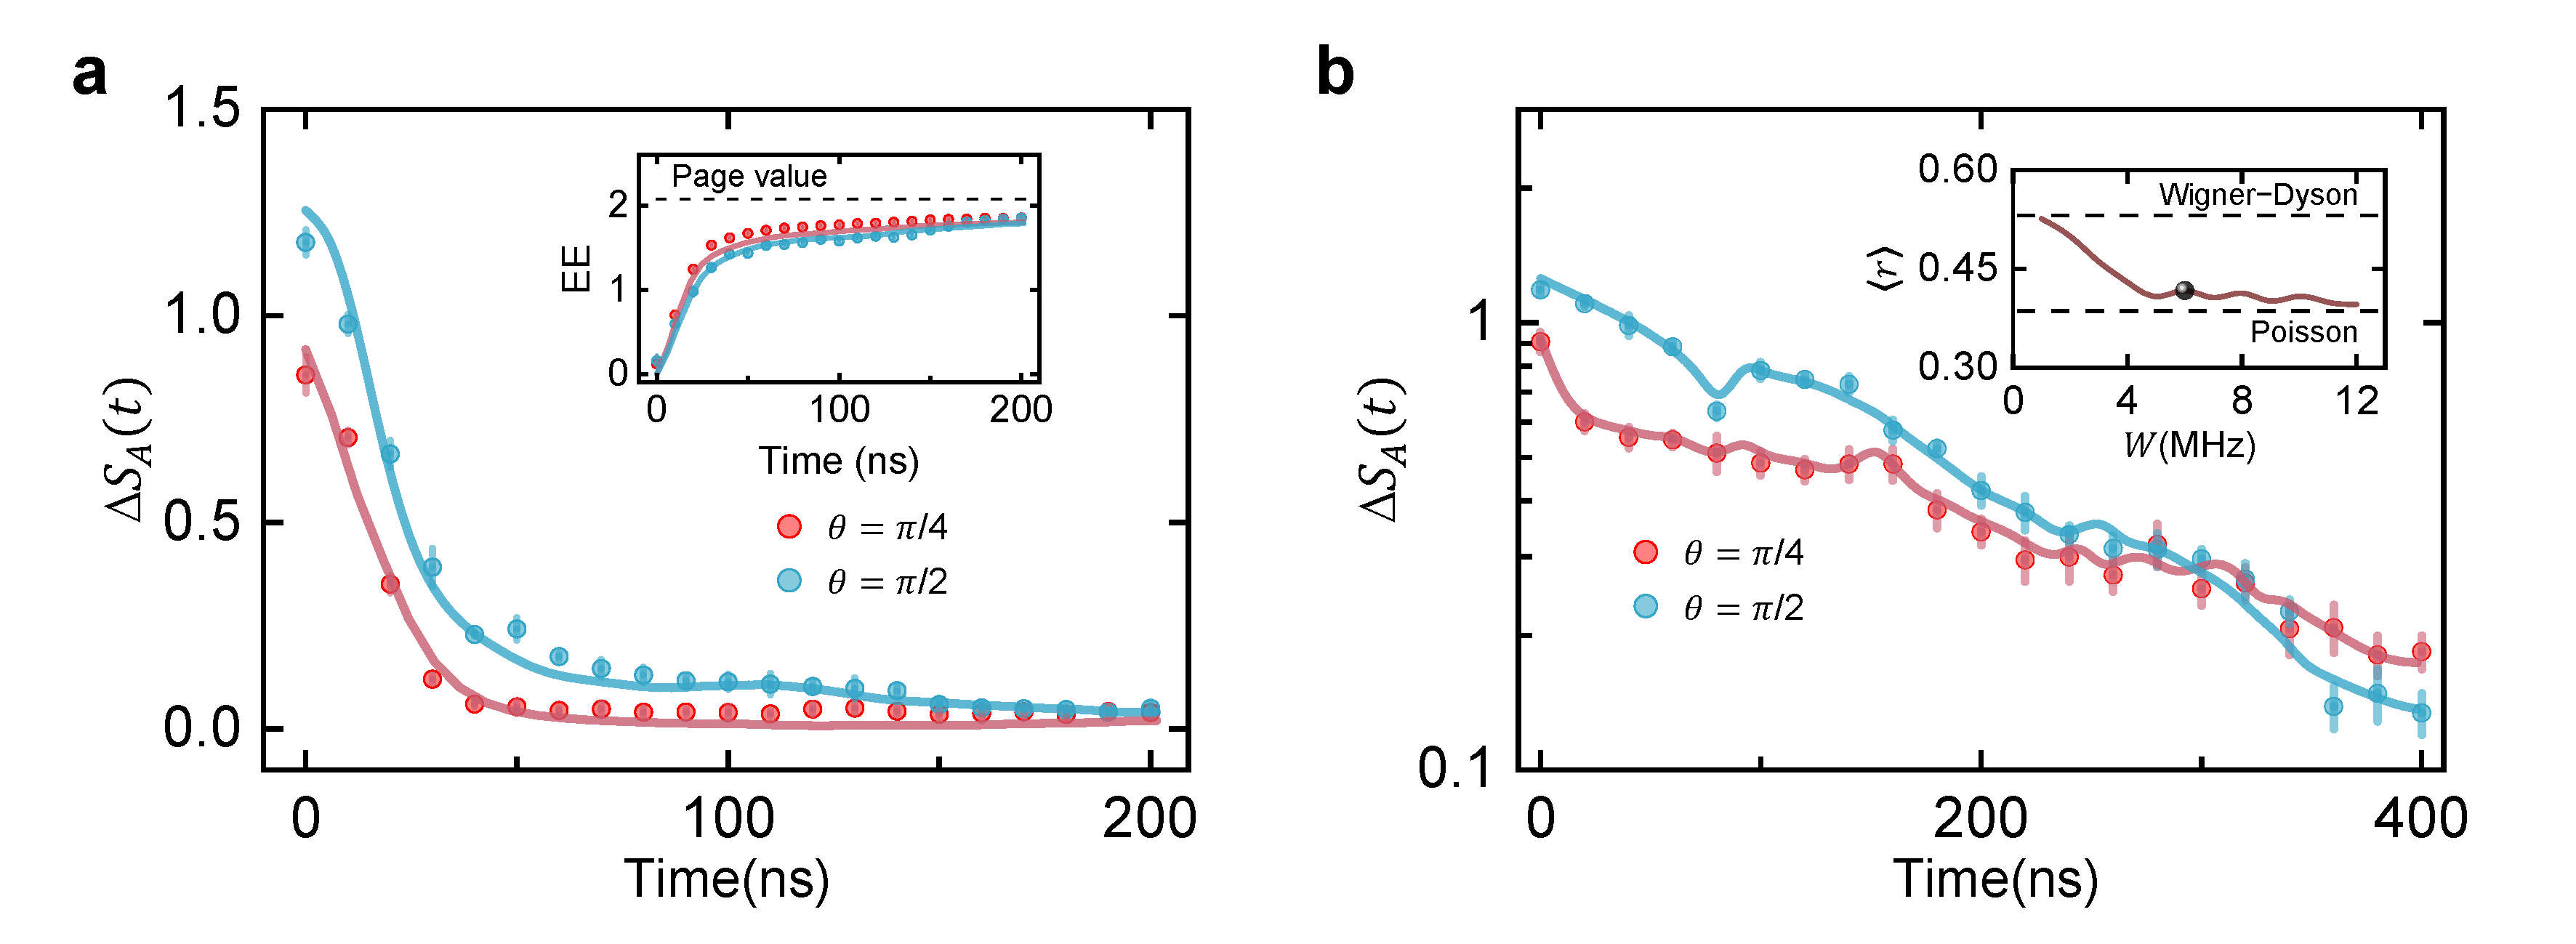
\includegraphics[width=0.95\textwidth]{Figure3/Figure3.pdf}
    \caption{
        \textcolor{blue}{中间耦合区间($r \approx 1$)的EA动力学。}
        (a) 共振条件下倾斜Néel态的EA动力学,显示$\theta = \pi/2$的态对称性恢复更慢,导致QME抑制。
        插图为纠缠熵动力学,显示两个态都趋于Page值,表明系统热化。
        (b) 引入线性势($W = 6$ MHz)后EA动力学,显示QME重新出现。
        插图为平均能级间距比$\langle r \rangle$随$W$的变化,表明系统从热化相向局域化相转变。
    }
    \label{fig:intermediate_coupling}
\end{figure}

\textcolor{blue}{图~\ref{fig:intermediate_coupling}(a)}的主图和插图都是红色线更快,说明对称性恢复的速度与热化速度成正相关。插图的红蓝线刚开始都是呈现线性增长。主图刚开始呈现线性下降。\textcolor{magenta}{EA与EE配合说明,相互验证。}
我们的研究结果不仅证明了灵活调控耦合构型可以实现QME的可调谐操控,而且阐明了系统对称性的恢复与热化动力学之间的密切联系。


\textcolor{blue}{关于热化:}
热吉布斯系综是描述系统在热平衡状态下的统计分布。

\textcolor{blue}{关于Page value:}
根据ETH,非可积量子系统的子系统behaves like一个随机态,纠缠熵趋于一个Page value。

\textcolor{red}{Page value:}一个随机纯态中,子系统的纠缠熵的平均值。

\begin{equation}
\left\langle S_A\right\rangle_{\mathrm{Page}} \approx \ln (2) \times \min \left(N_A, N_B\right)-\frac{1}{2} \times \frac{2^{\min \left(N_A, N_B\right)}}{2^{\max \left(N_A, N_B\right)}}
\end{equation}

对于本文的总系统$N=14$,子系统$A=3$,剩余系统$B=11$,$\min \left(N_A, N_B\right) = 3$,$\max \left(N_A, N_B\right) = 11$。

因此,Page value为:
\begin{equation}
\left\langle S_A\right\rangle_{\mathrm{Page}} \approx \ln (2) \times 3-\frac{1}{2} \times \frac{2^{3}}{2^{11}} \approx 2.08
\end{equation}

类似于经典热力学由温度确定的平衡态,量子多体系统由Page value确定纠缠熵。


\textcolor{blue}{主要观测现象:}
\begin{itemize}
    \item \textcolor{blue}{QME抑制}:在中间耦合区间,更大的初始对称性破缺($\theta = \pi/2$)导致\textcolor{blue}{更慢}的对称性恢复
    \item \textcolor{blue}{无动力学交叉}:EA曲线单调衰减,没有出现强短程耦合区间中的交叉现象
    \item \textcolor{blue}{热化特征}:纠缠熵线性增长并趋于Page值,表明系统达到热平衡
\end{itemize}

\subsection{物理机制解释}
\begin{itemize}
    \item \textcolor{blue}{热化主导}:中间耦合强度破坏了系统的可积性,使动力学由热化过程主导
    \item \textcolor{blue}{对称性恢复与热化的关联}:对称性恢复速率与热化速率正相关
    \item \textcolor{blue}{倾斜角效应}:较小倾斜角($\theta = \pi/4$)的态热化更快,因此对称性恢复也更快
    \item \textcolor{blue}{与强短程耦合的对比}:在可积性主导的强短程耦合中,准粒子机制导致反常动力学;在热化主导的中间耦合中,系统遵循正常的热化行为
\end{itemize}

\subsection{理论验证}
通过计算纠缠熵动力学验证热化假设:
\begin{itemize}
    \item 两个初始态的EE都增长并接近Page值
    \item EE的演化与EA动力学密切相关
    \item 较小倾斜角的态表现出更快的EE增长,对应更快的热化速率
\end{itemize}

\subsection{重要意义}
\begin{itemize}
    \item 首次实验展示了通过调节耦合强度可以实现QME的\textcolor{blue}{可控抑制}
    \item 阐明了对称性恢复与热化过程之间的\textcolor{blue}{内在联系}
    \item 为理解量子多体系统中非平衡动力学提供了重要见解
    \item 展示了超导量子处理器在研究多体物理中的强大能力
\end{itemize}

\textcolor{blue}{核心结论:}在中间耦合区间,热化过程主导系统动力学,导致QME被抑制。这表明QME的出现强烈依赖于系统的可积性和热化性质,为理解量子多体非平衡动力学提供了重要线索。


\section{QME的重现}

\subsection{研究背景与问题提出}
\begin{itemize}
    \item \textcolor{blue}{核心问题}:在中间耦合区间($r \approx 1$)热化抑制QME的情况下,能否通过系统调控重新激发QME?
    \item \textcolor{blue}{理论启示}:先前理论研究显示,热化抑制和遍历性破缺可导致QME在任意倾斜乘积态中出现
    \item \textcolor{blue}{实验策略}:利用系统的灵活性,通过两种独立机制恢复QME:
    \begin{enumerate}
        \item 引入在位线性势抑制热化
        \item 从倾斜铁磁态淬火映射到LMG模型
    \end{enumerate}
\end{itemize}

\subsection{机制一:在位线性势诱导的QME重现}

\subsubsection{实验设置}
\begin{itemize}
    \item \textcolor{blue}{在位势形式}:位置依赖线性势 $h_j/2\pi = W(7.5 - j)$,其中 $j=1,2,\ldots,14$
    \item \textcolor{blue}{势场强度}:$W = 6$ MHz
    \item \textcolor{blue}{耦合参数}:中间耦合区间($r \approx 1$)
    \item \textcolor{blue}{初始态}:倾斜Néel态($\theta = \pi/4$ 和 $\pi/2$)
\end{itemize}

\subsubsection{关键结果与物理机制}
\begin{figure}[H]
    \centering
    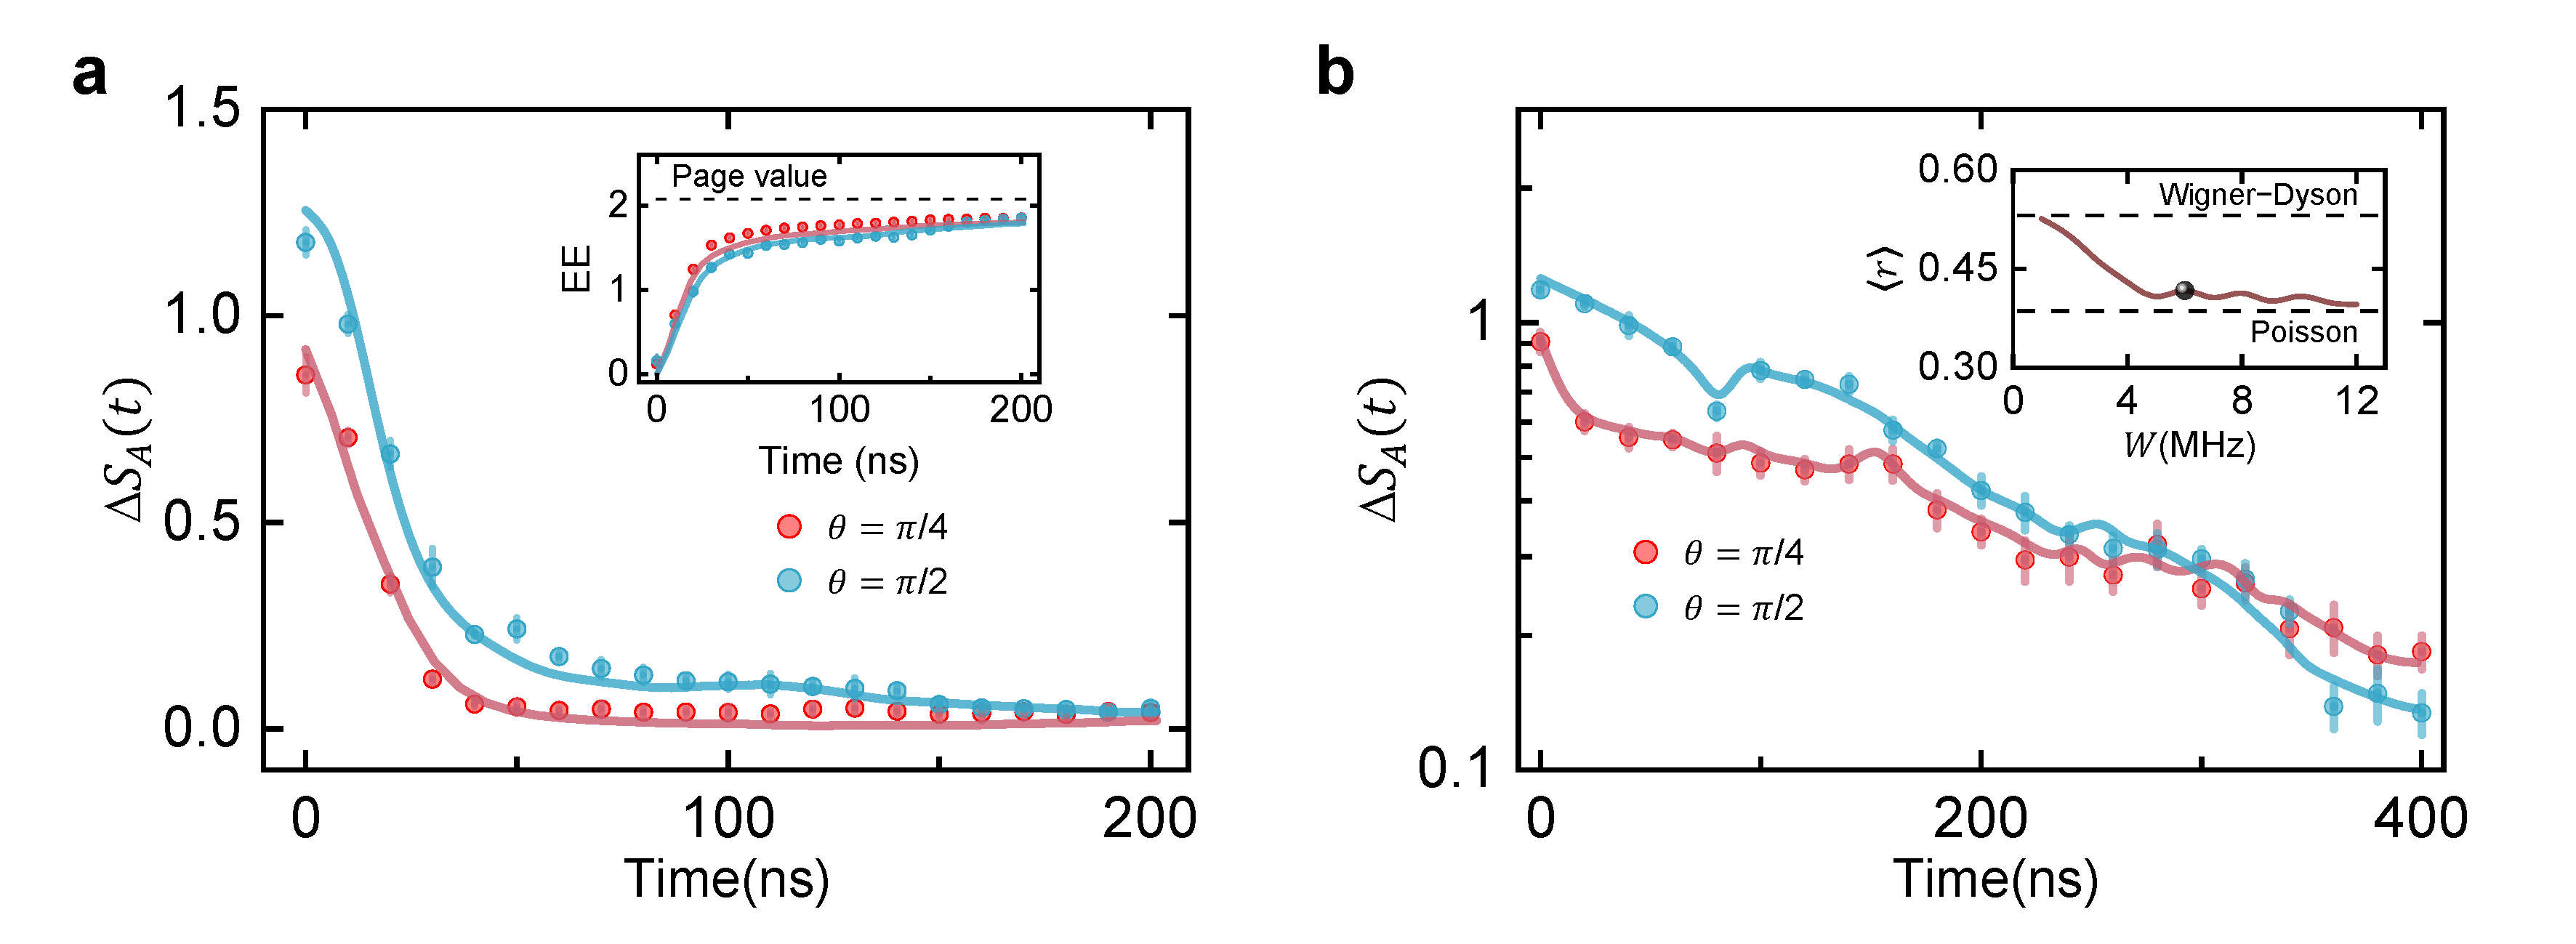
\includegraphics[width=0.95\textwidth]{Figure3/Figure3.pdf}
    \caption{
        \textcolor{blue}{在位线性势诱导的QME重现。}
        (b) 在位线性势($W = 6$ MHz)下倾斜Néel态的EA动力学,显示QME重现。
        插图为平均能级间距比$\langle r \rangle$随$W$的变化,表明系统从遍历相向局域化相转变。
    }
    \label{fig:QME_reemergence_linear}
\end{figure}

\textcolor{blue}{主要发现:}
\begin{itemize}
    \item \textcolor{blue}{对称性恢复的普遍减缓}:\textcolor{magenta}{线性势整体减慢了对称性恢复过程}
    \item \textcolor{blue}{角度依赖的抑制效应}:\textcolor{magenta}{对称性恢复的抑制程度随倾斜角变化,大角度$\theta$受抑制较弱}
    \item \textcolor{blue}{QME重现}:这种角度依赖的抑制导致EA曲线重新出现交叉,QME重现
\end{itemize}

\subsubsection{遍历性破缺的证据}
\begin{itemize}
    \item \textcolor{blue}{能级间距统计}:计算平均能级间距比$\langle r \rangle$:
    \[
    \langle r \rangle = \frac{1}{N}\sum_{n=1}^{N} \frac{\min(\delta_n, \delta_{n+1})}{\max(\delta_n, \delta_{n+1})}
    \]
    \item \textcolor{blue}{相变特征}:
    \begin{itemize}
        \item $W = 0$:$\langle r \rangle \approx 0.531$(Wigner-Dyson统计,遍历相)
        \item $W$增大:$\langle r \rangle \rightarrow 0.386$(Poisson统计,局域化相)
    \end{itemize}
    \item \textcolor{blue}{物理意义}:线性势诱导了遍历性破缺和局域化特征
\end{itemize}

\subsection{机制二:倾斜铁磁态淬火的QME重现}

\subsubsection{实验设置}
\begin{itemize}
    \item \textcolor{blue}{初始态}:倾斜铁磁态 $|\theta\rangle_F = (\cos\frac{\theta}{2}|0\rangle + \sin\frac{\theta}{2}|1\rangle)^{\otimes N}$
    \item \textcolor{blue}{耦合参数}:中间耦合区间($r \approx 1$)
    \item \textcolor{blue}{映射关系}:系统可映射到Lipkin-Meshkov-Glick (LMG)模型
\end{itemize}

\subsubsection{LMG模型映射理论}
\begin{itemize}
    \item \textcolor{blue}{集体自旋算符}:$\bm{S} = \sum_i \bm{\sigma}^i/2$
    \item \textcolor{blue}{有效哈密顿量}:
    \[
    H \approx \bar{g}(\bm{S}^2 - S_z^2) \rightarrow H_{\text{eff}} = -\bar{g}S_z^2
    \]
    \item \textcolor{blue}{动力学约束}:子系统动力学局限于$S_A = N_A/2$子空间
    \item \textcolor{blue}{EA简化关系}:$\Delta S_A(\theta,t) = C(\theta) - S_A(\theta,t)$
\end{itemize}

\subsubsection{实验结果与鲁棒性验证}
\begin{figure}[H]
    \centering
    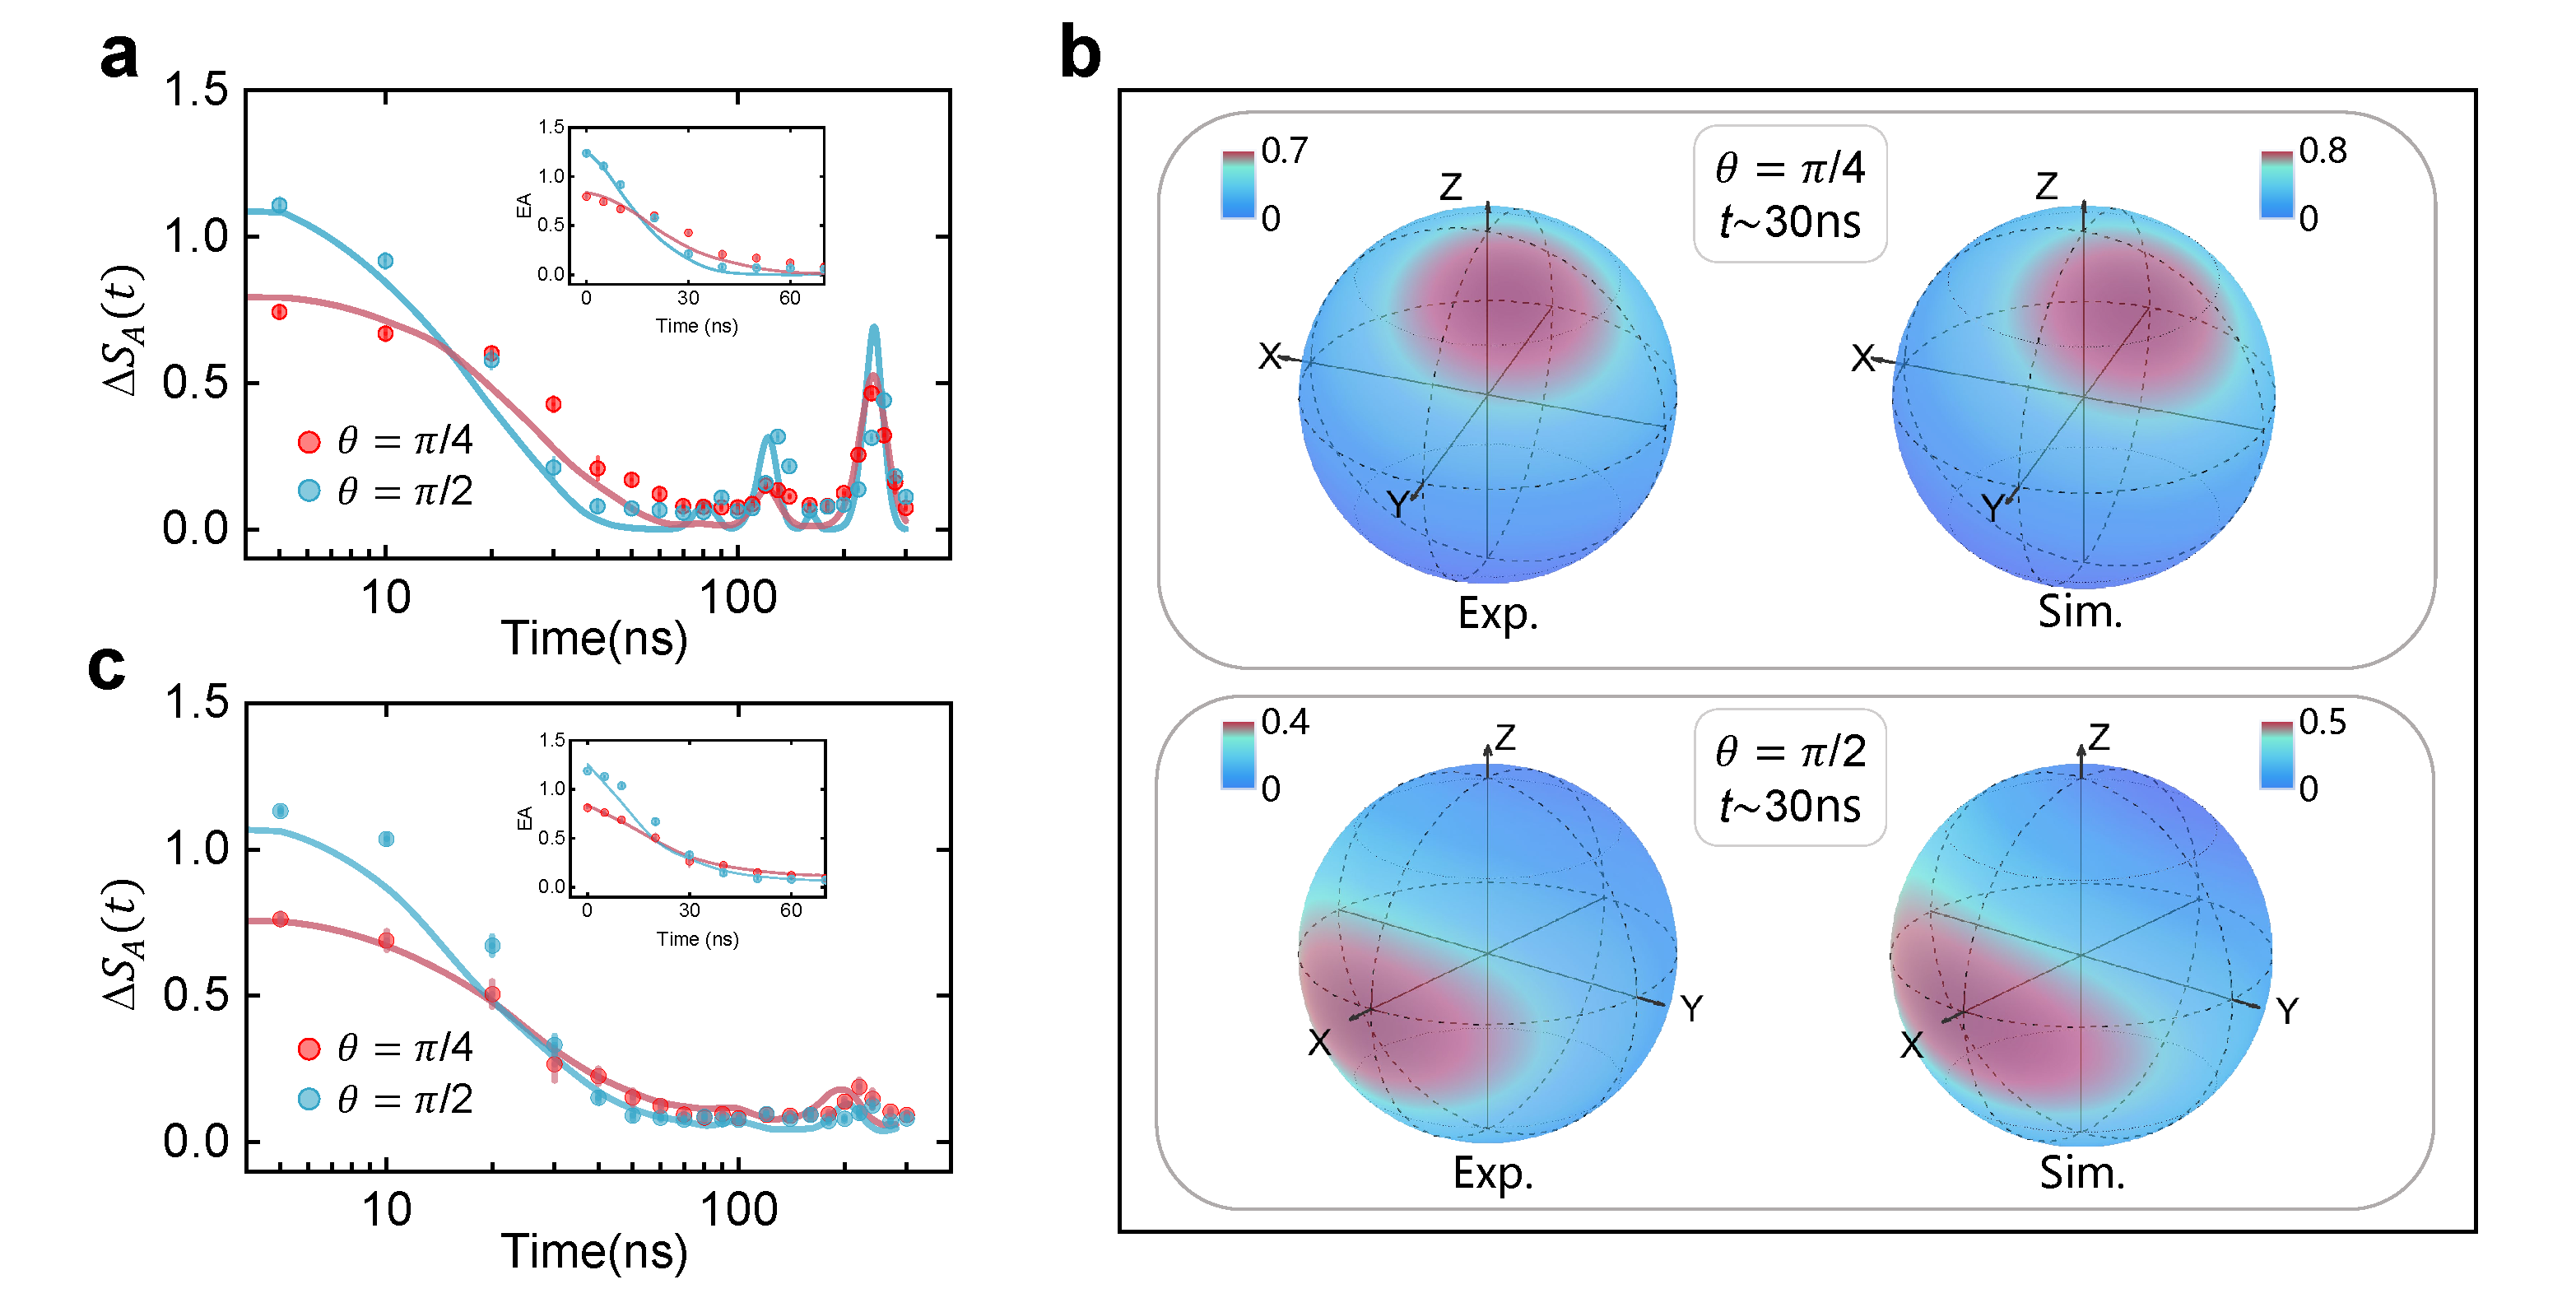
\includegraphics[width=0.95\textwidth]{Figure4/Figure4.pdf}
    \caption{
        \textcolor{blue}{倾斜铁磁态淬火的QME重现与鲁棒性。}
        (a) 共振条件下倾斜铁磁态的EA动力学,显示清晰的QME交叉和振荡行为。
        (b) 准分布函数$Q(\theta,\phi)$的演化,可视化对称性恢复过程。
        (c) 强在位无序下EA动力学,显示QME的鲁棒性。
    }
    \label{fig:QME_reemergence_FM}
\end{figure}

\textcolor{blue}{关键发现:}
\begin{itemize}
    \item \textcolor{blue}{QME重现}:倾斜铁磁态淬火在中间耦合区间重现QME,伴随特征振荡
    \item \textcolor{blue}{周期行为}:EA振荡周期$T_{\text{EA}} = \pi/\bar{g}$,完全复兴周期$T_S = 2\pi/\bar{g}$
    \item \textcolor{blue}{无序鲁棒性}:在强在位无序下($h_i/2\pi \in [-14\bar{g}, 14\bar{g}]$),QME交叉现象仍然存在
    \item \textcolor{blue}{与先前研究对比}:相比幂律XX自旋链($\alpha \approx 1$),本文的完全长程相互作用($\alpha = 0$)在实验时间尺度内产生更快的EA交叉
\end{itemize}

\subsection{物理机制总结}

\subsubsection{在位线性势机制}
\begin{itemize}
    \item \textcolor{blue}{核心机制}:通过抑制热化和诱导局域化特征,调制对称性恢复速率
    \item \textcolor{blue}{角度选择性}:大倾斜角态受热化抑制影响较小,导致非单调的对称性恢复动力学
    \item \textcolor{blue}{长时行为}:随着$W$增大,$\Delta S_A(\pi/4, t\rightarrow\infty)$上升而$\Delta S_A(\pi/2, t\rightarrow\infty)$基本不变,保证交叉出现
\end{itemize}

\subsubsection{倾斜铁磁态机制}
\begin{itemize}
    \item \textcolor{blue}{核心机制}:通过集体自旋动力学映射到可积的LMG模型
    \item \textcolor{blue}{动力学约束}:子系统局限于最大自旋子空间,导致$\rho_{A,Q}$时间无关
    \item \textcolor{blue}{可视化理解}:准分布函数$Q(\theta,\phi)$的方位角分布平坦化直接反映$U(1)$对称性恢复
\end{itemize}

\subsection{重要意义与结论}
\begin{itemize}
    \item \textcolor{blue}{多维调控能力}:展示了通过耦合强度、在位势和初始态选择对QME进行灵活调控的能力
    \item \textcolor{blue}{普适控制手段}:揭示了相互作用范围、势场工程和初始态选择作为非平衡动力学的通用控制手段
    \item \textcolor{blue}{平台优势}:凸显了全连接可调耦合超导量子处理器在研究量子多体动力学中的独特优势
    \item \textcolor{blue}{潜在应用}:为量子信息应用(如加速态制备和可控热化)开辟了新途径
\end{itemize}

\textcolor{blue}{核心结论:}通过两种独立机制——在位线性势诱导的热化抑制和倾斜铁磁态映射到LMG模型——在中间耦合区间成功实现了QME的重现,证明了QME作为非平衡量子动力学特征的普适性和可控性。


% ————— 个人笔记与 TODO —————
\section{个人笔记 }
\textcolor{blue}{什么是本征?}
“本征”这个词源于德语“eigen”,意思是“自己的”、“固有的”、“特征的”。
\textcolor{red}{本征方程}是指一个线性算子作用在本征态上时,其结果等于\textcolor{red}{本征值}乘以\textcolor{red}{本征态}本身。形式上,设$\hat{A}$是一个线性算子,$| \psi \rangle$是$\hat{A}$的本征向量,$\lambda$是$\hat{A}$在$| \psi \rangle$上的本征值,则有:
\begin{equation}
\hat{A} | \psi \rangle = \lambda | \psi \rangle
\end{equation}

\textcolor{red}{物理意义:}
如果一个系统处于算符 $\hat{A}$ 的某个本征态上,那么你测量这个物理量 $\hat{A}$ 时,会得到一个确定无疑的结果,这个结果就是对应的本征值。


\section{安德森局域化与多体局域化的区别}

\subsection{基本概念对比}

\begin{table}[H]
\centering
\caption{安德森局域化与多体局域化的核心区别}
\begin{tabular}{|p{0.45\textwidth}|p{0.45\textwidth}|}
\hline
\textcolor{blue}{安德森局域化 (Anderson Localization)} & \textcolor{blue}{多体局域化 (Many-Body Localization)} \\
\hline
\hline
\textcolor{blue}{研究对象}:\textcolor{blue}{非相互作用}粒子在无序势场中 & \textcolor{blue}{研究对象}:\textcolor{blue}{相互作用}量子多体系统在无序环境中 \\
\hline
\textcolor{blue}{发现时间}:1958年(Philip W. Anderson) & \textcolor{blue}{理论提出}:2006年左右(Basko, Aleiner, Altshuler等) \\
\hline
\textcolor{blue}{物理图像}:单个粒子被无序势场"囚禁" & \textcolor{blue}{物理图像}:整个多体系统被冻结,无法热化 \\
\hline
\end{tabular}
\end{table}

\subsection{物理机制对比}

\begin{table}[H]
\centering
\caption{物理机制与理论描述对比}
\begin{tabular}{|p{0.45\textwidth}|p{0.45\textwidth}|}
\hline
\textcolor{blue}{安德森局域化} & \textcolor{blue}{多体局域化} \\
\hline
\hline
\textcolor{blue}{局域化机制}:量子相干背散射导致波函数指数衰减 & \textcolor{blue}{局域化机制}:存在\textcolor{blue}{局域守恒量} $\tau_i^z$,系统记忆初始信息 \\
\hline
\textcolor{blue}{数学描述}:单粒子薛定谔方程 & \textcolor{blue}{数学描述}:多体哈密顿量,存在准局域积分运动常数 \\
\hline
\textcolor{blue}{波函数行为}:$|\psi(r)| \sim e^{-r/\xi}$(指数局域) & \textcolor{blue}{本征态特性}:面积律纠缠,不满足本征态热化假设 \\
\hline
\textcolor{blue}{维度依赖性}:在一维和二维中总是发生 & \textcolor{blue}{维度依赖性}:在一维和二维中稳定存在,三维存在争议 \\
\hline
\end{tabular}
\end{table}

\subsection{热化行为与动力学对比}

\begin{table}[H]
\centering
\caption{热化行为与动力学特性对比}
\begin{tabular}{|p{0.45\textwidth}|p{0.45\textwidth}|}
\hline
\textcolor{blue}{安德森局域化} & \textcolor{blue}{多体局域化} \\
\hline
\hline
\textcolor{blue}{热化行为}:不涉及热化概念(单粒子问题) & \textcolor{blue}{热化行为}:\textcolor{blue}{违反本征态热化假设(ETH)},不热化 \\
\hline
\textcolor{blue}{守恒量}:只有能量守恒 & \textcolor{blue}{守恒量}:有\textcolor{blue}{无限多局域守恒量} $\{\tau_i^z\}$ \\
\hline
\textcolor{blue}{纠缠熵}:不适用(单粒子无纠缠) & \textcolor{blue}{纠缠熵}:面积律缩放(与系统边界成正比) \\
\hline
\textcolor{blue}{记忆效应}:粒子位置被记忆 & \textcolor{blue}{记忆效应}:初始局域密度分布等信息被长期记忆 \\
\hline
\textcolor{blue}{输运性质}:扩散被完全抑制,电导率为零 & \textcolor{blue}{动力学行为}:局域可观测量不弛豫到热平衡值 \\
\hline
\end{tabular}
\end{table}

\subsection{实验特征与探测方法对比}

\begin{table}[H]
\centering
\caption{实验特征与探测方法对比}
\begin{tabular}{|p{0.45\textwidth}|p{0.45\textwidth}|}
\hline
\textcolor{blue}{安德森局域化} & \textcolor{blue}{多体局域化} \\
\hline
\hline
\textcolor{blue}{实验平台}:电子输运、冷原子、波导阵列 & \textcolor{blue}{实验平台}:超冷原子、离子阱、超导量子比特 \\
\hline
\textcolor{blue}{探测信号}:电导率、扩散系数、波函数成像 & \textcolor{blue}{探测信号}:纠缠熵、不平衡度、能级统计 \\
\hline
\textcolor{blue}{能级统计}:泊松分布 & \textcolor{blue}{能级统计}:泊松分布($\langle r \rangle \approx 0.386$) \\
\hline
\textcolor{blue}{在你论文中的体现}:不直接相关 & \textcolor{blue}{在你论文中的体现}:通过$\langle r \rangle$从0.53→0.39探测MBL转变 \\
\hline
\end{tabular}
\end{table}

\subsection{理论意义与物理内涵对比}

\begin{table}[H]
\centering
\caption{理论意义与物理内涵对比}
\begin{tabular}{|p{0.45\textwidth}|p{0.45\textwidth}|}
\hline
\textcolor{blue}{安德森局域化} & \textcolor{blue}{多体局域化} \\
\hline
\hline
\textcolor{blue}{理论意义}:量子 coherent 背散射的经典范例 & \textcolor{blue}{理论意义}:提供了在孤立量子系统中避免热化的机制 \\
\hline
\textcolor{blue}{对统计物理的挑战}:无直接挑战 & \textcolor{blue}{对统计物理的挑战}:\textcolor{blue}{颠覆传统统计物理基础} \\
\hline
\textcolor{blue}{应用前景}:电子器件、光子学 & \textcolor{blue}{应用前景}:量子信息存储、量子计算保护 \\
\hline
\textcolor{blue}{相变特性}:金属-绝缘体转变 & \textcolor{blue}{相变特性}:MBL相-热化相转变 \\
\hline
\end{tabular}
\end{table}

\subsection{关键物理洞察}

\begin{itemize}
\item \textcolor{blue}{安德森局域化是MBL的基础}:MBL可以看作是安德森局域化在相互作用系统中的推广

\item \textcolor{blue}{相互作用的双重角色}:
\begin{itemize}
\item 弱相互作用可能破坏安德森局域化
\item 但强无序下,系统仍能保持局域化(MBL相)
\end{itemize}

\item \textcolor{blue}{在你的论文中的体现}:
\begin{itemize}
\item 图3b中的线性势诱导了类似MBL的行为
\item 通过$\langle r \rangle$的测量来量化遍历性破缺程度
\item 这为理解QME的重现提供了理论基础
\end{itemize}

\item \textcolor{blue}{根本区别的核心}:
\begin{itemize}
\item 安德森局域化:\textcolor{blue}{单粒子}在无序中的定域化
\item 多体局域化:\textcolor{blue}{整个量子多体系统}避免热化的机制
\end{itemize}
\end{itemize}

\subsection{总结}

\textcolor{blue}{安德森局域化}和\textcolor{blue}{多体局域化}虽然都涉及无序诱导的局域化现象,但它们在物理本质、理论框架和实验表现上存在根本区别。理解这一区别对于把握现代凝聚态物理中热化与局域化的竞争关系至关重要,也是理解你论文中通过调节在位势来操控量子动力学的基础。

\subsection{Wigner-Dyson分布的物理起源}
\begin{itemize}
    \item \textbf{核心机制}:\textbf{能级排斥}
    \item \textbf{物理图像}:在量子混沌系统中,不同本征态之间强烈混合,导致能级"相互排斥"
    \item \textbf{数学表达}:对于高斯正交系综(GOE):
    \[
    P(s) = \frac{\pi s}{2} e^{-\pi s^2/4}
    \]
    \item \textbf{特征}:
    \begin{itemize}
        \item 小间距概率$P(s \rightarrow 0) \rightarrow 0$
        \item 平均能级间距比:$\langle r \rangle \approx 0.53$
    \end{itemize}
\end{itemize}


\subsection{Poisson分布的物理起源}
\begin{itemize}
    \item \textbf{核心机制}:\textbf{能级随机分布}
    \item \textbf{物理图像}:在局域化系统中,不同空间区域的能级独立变化
    \item \textbf{数学表达}:
    \[
    P(s) = e^{-s}
    \]
    \item \textbf{特征}:
    \begin{itemize}
        \item 小间距概率$P(s \rightarrow 0) \rightarrow 1$
        \item 平均能级间距比:$\langle r \rangle \approx 0.386$
    \end{itemize}
\end{itemize}

\subsection{可积系统的能级统计}
\begin{itemize}
    \item \textbf{重要结论}:\textbf{可积系统通常也满足Poisson统计}
    \item \textbf{物理原因}:
    \begin{itemize}
        \item 可积系统有大量守恒量,能级可以按不同量子数分类
        \item 在同一对称性子空间内,能级通常没有排斥
        \item 因此表现出类似随机分布的统计特性
    \end{itemize}
    \item \textbf{与MBL的区别}:
    \begin{itemize}
        \item \textbf{可积系统}:由于守恒量导致的准独立模式
        \item \textbf{MBL系统}:由于无序导致的局域化
        \item \textbf{结果相同}:都表现为Poisson统计
    \end{itemize}
\end{itemize}

\subsection{在量子Mpemba效应研究中的体现}
\begin{itemize}
    \item \textbf{中间耦合区间(热化相)}:
    \begin{itemize}
        \item $\langle r \rangle \approx 0.53$(Wigner-Dyson)
        \item 系统充分热化,QME被抑制
    \end{itemize}
    
    \item \textbf{引入线性势(局域化相)}:
    \begin{itemize}
        \item $\langle r \rangle \rightarrow 0.39$(Poisson)
        \item 热化被抑制,QME重新出现
    \end{itemize}
    
    \item \textbf{物理意义}:能级统计作为系统是否热化的\textbf{诊断工具}
\end{itemize}

\subsection{随机矩阵理论框架}
\begin{itemize}
    \item \textbf{Wigner-Dyson分布}:描述\textbf{没有特殊结构的随机矩阵}
    \begin{itemize}
        \item 矩阵元随机且相互关联
        \item 代表高度混合的量子系统
    \end{itemize}
    
    \item \textbf{Poisson分布}:描述\textbf{对角占优或块对角的矩阵}
    \begin{itemize}
        \item 矩阵近似对角化或块对角化
        \item 代表可积或局域化系统
    \end{itemize}
\end{itemize}


\subsection{不同量子相的能级统计特征}
\begin{table}[H]
\centering
\begin{tabular}{|l|c|c|}
\hline
\textbf{量子相} & \textbf{能级统计} & \textbf{物理机制} \\
\hline
\textbf{量子混沌/遍历相} & Wigner-Dyson ($\langle r \rangle \approx 0.53$) & 能级排斥,强耦合 \\
\hline
\textbf{多体局域化相} & Poisson ($\langle r \rangle \approx 0.386$) & 局域守恒量,能级独立 \\
\hline
\textbf{可积系统} & Poisson ($\langle r \rangle \approx 0.386$) & 大量守恒量,能级分类 \\
\hline
\textbf{临界点} & 中间分布 & 相变区域的普适类 \\
\hline
\end{tabular}
\end{table}

\subsection{能级统计的深层物理意义}
\begin{itemize}
    \item \textbf{热化的微观基础}:Wigner-Dyson统计是本征态热化假设(ETH)的体现
    \item \textbf{量子混沌的标志}:能级排斥反映了经典混沌在量子系统中的对应
    \item \textbf{普适性}:这些统计规律与具体哈密顿量细节无关,只依赖于对称性和基本性质
    \item \textbf{在你研究中的应用}:
    \begin{itemize}
        \item 通过$\langle r \rangle$量化系统的热化程度
        \item 为QME的出现和抑制提供微观解释
        \item 连接了宏观动力学(对称性恢复)与微观统计(能级分布)
    \end{itemize}
\end{itemize}


\section{不可热化系统的完整分类}

\subsection{传统不可热化系统}

\begin{table}[H]
\centering
\caption{主要不可热化系统类型}
\begin{tabular}{|p{0.3\textwidth}|p{0.3\textwidth}|p{0.3\textwidth}|}
\hline
\textbf{系统类型} & \textbf{物理机制} & \textbf{能级统计} \\
\hline
\textbf{可积系统} & 存在大量守恒量 & Poisson ($\langle r \rangle \approx 0.386$) \\
\hline
\textbf{多体局域化(MBL)} & 强无序导致局域守恒量 & Poisson ($\langle r \rangle \approx 0.386$) \\
\hline
\textbf{量子多体疤痕} & 动力学约束与特殊对称性 & 混合分布 \\
\hline
\textbf{拓扑有序态} & 拓扑保护,简并基态 & 依赖于具体系统 \\
\hline
\textbf{量子时间晶体} & 时间平移对称性自发破缺 & 特殊周期性结构 \\
\hline
\end{tabular}
\end{table}

\subsection{量子多体疤痕}

\subsubsection{物理机制}
\begin{itemize}
    \item \textbf{核心特征}:在量子混沌系统中存在\textbf{特殊的不热化轨道}
    \item \textbf{物理图像}:类似于经典动力学中的周期轨道在量子系统中的对应
    \item \textbf{典型模型}:PXP模型(Rydberg原子链)
    \[
    H = \sum_i P_{i-1} \sigma^x_i P_{i+1}
    \]
    \item \textbf{动力学表现}:初始态在特殊子空间中演化,表现出周期性复兴
\end{itemize}

\subsubsection{与MBL的区别}
\begin{itemize}
    \item \textbf{MBL}:所有初始态都不热化
    \item \textbf{量子疤痕}:只有特定初始态不热化,其他态正常热化
    \item \textbf{能级统计}:整体系统是Wigner-Dyson,但疤痕态有特殊结构
\end{itemize}

\subsection{拓扑有序态}

\subsubsection{物理机制}
\begin{itemize}
    \item \textbf{核心特征}:拓扑简并基态,受拓扑保护
    \item \textbf{典型例子}:
    \begin{itemize}
        \item 分数量子霍尔态
        \item 自旋液体
        \item 拓扑超导体
    \end{itemize}
    \item \textbf{热化行为}:在能隙以上可能热化,但拓扑基态本身不热化
\end{itemize}

\subsubsection{具体表现}
\begin{itemize}
    \item \textbf{拓扑简并}:基态简并度依赖于系统拓扑(如环面 genus)
    \item \textbf{拓扑保护}:局域扰动不能混合不同的拓扑 sector
    \item \textbf{长程纠缠}:具有拓扑纠缠熵
\end{itemize}

\subsection{量子时间晶体}

\subsubsection{物理机制}
\begin{itemize}
    \item \textbf{核心特征}:时间平移对称性自发破缺
    \item \textbf{两种类型}:
    \begin{itemize}
        \item \textbf{离散时间晶体}:在周期驱动下表现出倍周期响应
        \item \textbf{连续时间晶体}:在连续时间演化中自发振荡
    \end{itemize}
    \item \textbf{热化行为}:违反Floquet热化假设,保持周期性动力学
\end{itemize}

\subsection{其他特殊类型}

\subsubsection{Stark多体局域化}
\begin{itemize}
    \item \textbf{机制}:由线性梯度场(而非随机无序)诱导的局域化
    \item \textbf{在你论文中的体现}:图3b中的线性势$W(7.5-j)$就属于这种类型
    \item \textbf{特点}:不需要随机无序,仅靠线性势就能抑制热化
\end{itemize}

\subsubsection{准周期系统}
\begin{itemize}
    \item \textbf{机制}:准周期势(如Aubry-André模型)诱导的局域化
    \item \textbf{与随机无序的区别}:具有更丰富的相图,可能存在迁移率边缘
\end{itemize}

\subsubsection{约束系统}
\begin{itemize}
    \item \textbf{机制}:动力学约束限制希尔伯特空间的探索
    \item \textbf{例子}:倾斜场中的Ising模型、Fracton体系
    \item \textbf{表现}:系统只能访问希尔伯特空间的子集
\end{itemize}

\subsection{在你论文中的具体联系}

\subsubsection{线性势与Stark MBL}
\begin{itemize}
    \item 你论文中的线性势$h_j/2\pi = W(7.5-j)$正是\textbf{Stark MBL}的典型设置
    \item 这解释了为什么在引入线性势后,系统从热化相转变为局域化相
    \item $\langle r \rangle$从0.53→0.39证实了这一转变
\end{itemize}

\subsubsection{QME重现的深层意义}
\begin{itemize}
    \item \textbf{可积系统}:准粒子机制导致QME
    \item \textbf{热化系统}:QME被抑制
    \item \textbf{局域化系统}:热化被抑制,QME重新出现
    \item 这展示了QME作为\textbf{热化诊断工具}的价值
\end{itemize}

\subsection{理论框架:ETH的违反}

\begin{itemize}
    \item \textbf{本征态热化假设(ETH)}:所有本征态都是"热态"
    \item \textbf{ETH的违反条件}:
    \begin{itemize}
        \item 可积系统:守恒量导致能级分类
        \item MBL:局域守恒量阻止热化
        \item 量子疤痕:特殊对称性保护特定轨道
        \item 拓扑序:拓扑保护阻止态混合
    \end{itemize}
    \item \textbf{共同特征}:系统无法探索整个希尔伯特空间
\end{itemize}

\subsection{实验探测方法}

\begin{table}[H]
\centering
\caption{不同不可热化系统的实验特征}
\begin{tabular}{|p{0.25\textwidth}|p{0.35\textwidth}|p{0.3\textwidth}|}
\hline
\textbf{系统类型} & \textbf{关键实验信号} & \textbf{在你论文中的对应} \\
\hline
\textbf{可积系统} & 纠缠熵亚线性增长,不达Page值 & 图2c的QME现象 \\
\hline
\textbf{MBL} & 不平衡度不衰减,$\langle r \rangle \approx 0.39$ & 图3b的$\langle r \rangle$测量 \\
\hline
\textbf{量子疤痕} & 特定初始态的周期性复兴 & 未直接研究 \\
\hline
\textbf{拓扑序} & 拓扑纠缠熵,任意子统计 & 超出当前研究范围 \\
\hline
\textbf{时间晶体} & 倍周期响应,长期相干 & 未直接研究 \\
\hline
\end{tabular}
\end{table}

\subsection{总结}

\textbf{不可热化系统的完整图像}:

\begin{itemize}
    \item \textbf{传统类型}:可积系统、多体局域化
    \item \textbf{新兴类型}:量子疤痕、拓扑序、时间晶体
    \item \textbf{共同本质}:违反本征态热化假设(ETH)
    \item \textbf{在你研究中的体现}:
    \begin{itemize}
        \item 通过调节耦合强度研究可积到热化的转变
        \item 通过引入势场研究热化到局域化的转变
        \item 系统展示了丰富的非平衡量子动力学相图
    \end{itemize}
\end{itemize}

这些不同类型的不可热化系统共同构成了量子多体物理中丰富的非平衡行为,为理解和操控量子动力学提供了多样化的平台。


\vfill
{\small 记录时间:\today\ \currenttime}

\end{document}